% -*- root: ../../main.tex -*- %
\subsection{Components} % (fold)
\label{sub:components}
  As noted in \ref{par:micro_services_architecture}, one of the downsides of \ac{MSA} is that suitable service boundaries have to be determined. Some sources advise to first build a monolithic application and then analyze the result to single out services that can be extracted. In case of \acp{WfMS}, the identification of system components by the \ac{WFMC} for their reference model can be interpreted as such an analysis. Based on those components further micro-services for the prototype are then identified.

  As presented in \ref{sub:system_components}, the \ac{WFMC} identified the following components:
    \begin{itemize}[nosep]
      \item Software Components
        \begin{itemize}[nosep]
          \item Definition Tool
          \item Organization Modeling Tool
          \item User Interface
          \item Workflow Engine(s)
          \item Worklists Handler
        \end{itemize}
      \item Data Components
        \begin{itemize}[nosep]
          \item Organization Data
          \item Process Definitions Data
          \item Workflow Control Data
          \item Workflow Relevant Data
          \item Worklists Data
        \end{itemize}
    \end{itemize}

    - ui adapted to suit the API gateway pattern
    - user interface split per purpose (dev/user)

  Besides the major components, independent functionalities which are frequently used may be singled out to own services. To demonstrate this exemplarily, a service which deals with the validation of input and output data is extracted for this prototype.

  In the following, the resulting set of services is presented.

    \subsubsection{Workflow Definition Service} % (fold)
      \label{subs:workflow_definition_service}

      The workflow definition service encompasses the functions envisioned by the \ac{WFMC} as Process Definition Tools, \ie it is concerned with the analysis, modeling, description and documentation of business processes in form of workflow models and their process definitions. It further manages the assignment of activities to roles.

      With regards to that functional scope, this is also the component that should handle the transformation of workflows into their distributable format, \eg a self-contained description file or Docker images. In case of the latter, the workflow definition service would require access to a Docker daemon in order to perform the export. Once a workflow is transformed, the service should publish it.

      This components needs to incorporate the concepts required for its task. That is, workflow, activity , process definition, and control flow. The roles assigned to activities have only to be dealt with as unique identifiers, relying on the assumption that components which have to use them may resolve them themselves.

      According to the concept of \ac{MSA}, the workflow definition service component does not bring its own user interface, but rather exposes only an \ac{API}. This allows workflow definitions to be created and altered by arbitrary other services, \eg some converting service which translates other process definition formats, some feedback mechanism that alters workflows based on their execution performance, or different gateways which provide suitable user interfaces for various user devices.
      % subsubsection workflow_definition_service (end)

    \subsubsection{Organization Management Service} % (fold)
      \label{subs:organization_management_service}
      The organization management service is part of the ``administration and monitoring tools''.
      As its name suggests, its functionality is aimed at the management of actors within an organization and their mutual relationships. Based this information, it may be queried for users or roles, or authenticate users for the use of the \ac{WfMS}. Just like the workflow definition service, this service only exposes an \ac{API}.
      % subsubsection organization_management_service (end)

    \subsubsection{Worklist Service} % (fold)
      \label{subs:worklist_service}
      The sole responsibility of this service is the management of users' worklists. It should create and delete worklist items on request and publish the data users submitted to it. If an user is deleted, it should reschedule the worklist item to a new provided user.
      % subsubsection worklist_service (end)

    \subsubsection{Workflow Engine Service} % (fold)
      \label{subs:workflow_engine_service}

      In wide parts, the workflow engine service is congruent to the ``workflow engine'' as identified by the \ac{WFMC} in terms of functionality. It is
      As its responsibilities encompass the provision of the runtime environment, the workflow engine service should instanciate a provisioner on a node when it is added to the swarm. It also should ensure, that

      - choose participants
      - add to execution networks

      The chosen option from the solutions presented in \ref{sec:docker_for_wf_execution} has an impact on the range of functionalities that this service has.

      The extent to which the workflow engine service controls the instanciation of workflow components depends on .
      % subsubsection workflow_engine_service (end)

    \subsubsection{Developer Gateway} % (fold)
      \label{subs:developer_gateway}



        - provides access to
          - infrastructure
          - definition
          - organization
      % subsubsection developer_gateway (end)

    \subsubsection{User Gateway} % (fold)
      \label{subs:user_gateway}
        - provides access to
          - worklists
          - forms
      % subsubsection user_gateway (end)

    \subsubsection{Organization Data} % (fold)
    \label{subs:organization_data}

    % subsubsection organization_data (end)
    \subsubsection{Process Definitions Data} % (fold)
    \label{subs:process_definitions_data}

    % subsubsection process_definitions_data (end)
    \subsubsection{Workflow Control Data} % (fold)
    \label{subs:workflow_control_data}

    % subsubsection workflow_control_data (end)
    \subsubsection{Workflow Relevant Data} % (fold)
    \label{subs:workflow_relevant_data}

    % subsubsection workflow_relevant_data (end)
    \subsubsection{Worklists Data} % (fold)
    \label{subs:worklists}

    % subsubsection worklists (end)

  \subsubsection{Validation Service} % (fold)
    \label{subs:valitation_service}
    One micro-service that might be extracted from the above services concerns the validation of data is the validation service. Given a dataset and a set of rules on how to validate this dataset, the service is able to perform its task autonomously. As validation is a frequently recurring action in the execution of workflows -- before and after each activity and workflow -- it could thus be beneficial to be able to scale the execution of this task independently.
    % subsubsection valitation_service (end)

  \subsubsection{Support Services} % (fold)
  \label{ssub:support_components}
    There are three services which are required for the infrastructure in order to achieve the specified objectives. First, some \ac{MOM}, as it enables the communication between all components. Second, a service that allows the configuration of the execution environment. And third, a component that takes care of provisioning all machines with the images they require.

    \subsubsection{Message Oriented Middleware} % (fold)
      \label{subs:message_oriented_middleware}
      - must be reachable by all other services
      % subsubsection message_oriented_middleware (end)

    \subsubsection{Infrastructure Management Service} % (fold)
      \label{subs:environment_management_service}

        - see machines in the swarm
        - see their (labelled) properties
        - see (running) containers and available images
      % subsubsection environment_management_service (end)

    \subsubsection{Registry} % (fold)
    \label{subs:registry}
      All solutions presented in Section~\ref{sec:docker_for_wf_execution} feature custom Docker images, be it workers or contanierized activities or workflows. These images presumably contain information on business processes and other information whose disclosure should be avoided.  In order to store and distribute these images, a private registry is thus required.

      A possible alternative for less sensitive images could be the utilization of a private remote repository on the Docker Hub.
    % subsubsection registry (end)

    \subsubsection{Provisioning Service} % (fold)
      \label{subs:provisioning_service}
        The objectives include the reduction of administrative work. In order to prevent the user from having to distribute the Docker images required for the execution of workflows manually, a service should perform this task. This service should provision each machine with said images whenever such an image is created or updated. If a workflow or an activity is deleted, the service should remove its respective image from all machines.

        The service could either run as an instance on each machine, performing the required Docker operations locally, or run on the Docker Swarm master machine as one instance and perform the operations remotely on all machines.
      % subsubsection provisioning_service (end)
  % subsubsection support_components (end)

  \begin{figure}[htbp]
    \centering
    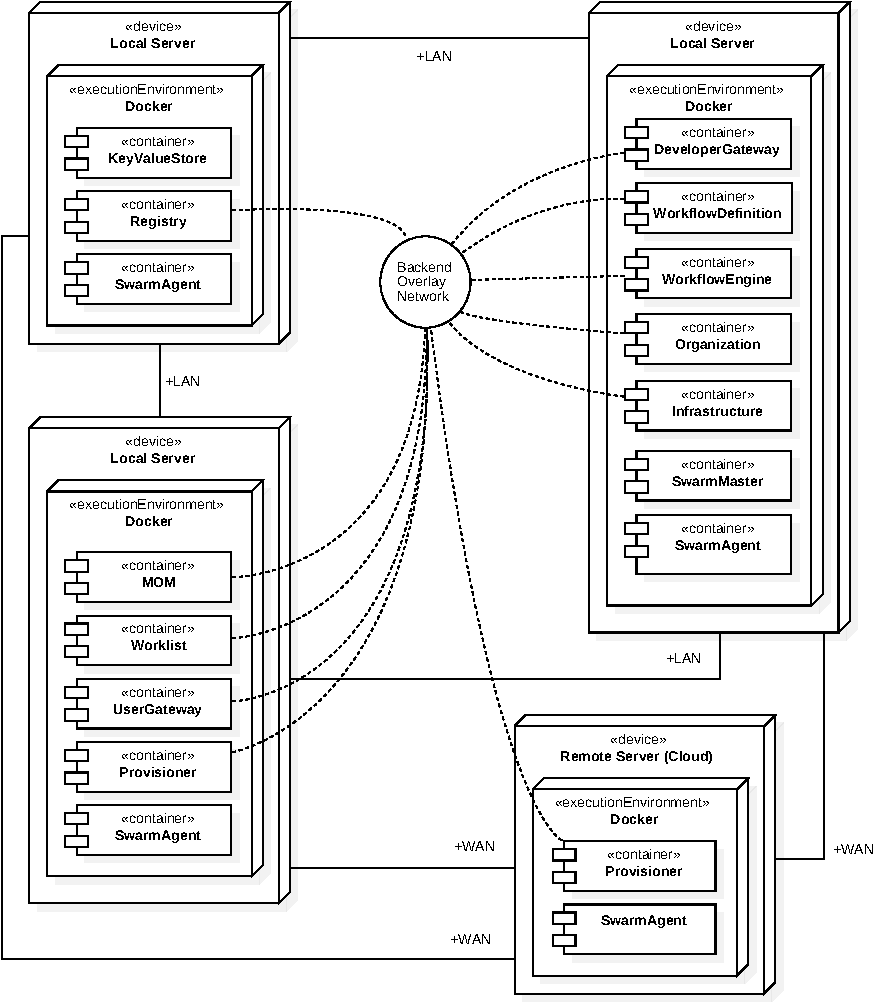
\includegraphics[width=0.95\textwidth]{content/images/Architecture-crop.pdf}
    \caption*{\scriptsize Note: the depicted distribution of containers to nodes is just exemplarily. Most of them could run on any node in the swarm. The only mandatory assignments are the swarm agents, of which each node needs one, and the provisioners, of which each node that is intended to execute workflows on needs one. \\ Also, the databases and their respective data volumes were omitted for the sake of clarity.}
    \caption{Deployment Diagram of the Architecture}
    \label{fig:label}
  \end{figure}
% subsection components (end)

\subsection{Communication} % (fold)
  \label{sub:application_level_communication}
  While the previous considerations were targeted at finding a model for the low-level communication, a way how the services communicate with each other

  - likeliness of scaling
  - REST between non-scaling services
  - MOM for broadcasts / asynchronous jobs

% subsection application_level_communication (end)

  % \begin{sequencediagram}
  % \newinst{u}{Developer Gateway}
  % \newinst[1]{d}{Definition Service}
  % \newinst[1]{m}{MOM}
  % \newinst[1]{p}{Provisioner}

  % \mess{u}{subscribe}{m}
  % \mess{d}{subscribe}{m}
  % \mess{p}{subscribe}{m}

  % \mess{u}{wfms.wf.create}{m}
  % \mess{m}{wfms.wf.create}{d}
  % \mess{d}{wfms.wf.created}{m}
  % \mess{m}{wfms.wf.created}{u}
  % \mess{u}{wfms.pd.update}{m}
  % \mess{m}{wfms.pd.update}{d}
  % \mess{d}{wfms.pd.updated}{m}
  % \mess{m}{wfms.pd.updated}{u}
  % \mess{u}{wfms.wf.export}{m}
  % \mess{m}{wfms.wf.export}{d}
  % \mess{d}{wfms.wf.exported}{m}
  % \mess{m}{wfms.wf.exported}{p}
  % \mess{m}{wfms.wf.exported}{u}

  % \end{sequencediagram}

% subsection inter_component_communication (end)
